\section{Analysis of the Numerical Results}
\label{sec:results}

\subsection{Classical Model Results}
\subsubsection{Leaderboard Results}

The per-model leaderboard (aggregating across all evaluated series) reveals several patterns:

\begin{enumerate}
    \item \textbf{Baselines are surprisingly competitive.} The Expanding Mean and Rolling Mean models often perform comparably to or better than fitted parametric models, reflecting the difficulty of beating simple forecasts on noisy financial data.
    \item \textbf{Low-order models tend to outperform high-order ones.} AR(1)--AR(3) generally outperform AR(7)--AR(10), consistent with the ACF analysis showing short-lag dominance.
    \item \textbf{MA(1) on differences is strong.} As the mathematical equivalent of Simple Exponential Smoothing, MA(1) is a robust performer.
\end{enumerate}

\subsubsection{The $d=0$ vs. $d=1$ Head-to-Head}

Comparing matched-order ARIMA pairs confirms the EDA's stationarity finding:
\begin{itemize}
    \item ARIMA($p$, 1, $q$) variants systematically outperform their ARIMA($p$, 0, $q$) counterparts.
    \item First differencing is genuinely load-bearing for this dataset.
\end{itemize}

\subsubsection{Per-Series Winner Analysis}

No single model dominates across all series. The per-series winner table shows considerable heterogeneity:
\begin{itemize}
    \item Some series are best served by simple baselines (Naive, Expanding Mean).
    \item Others benefit from low-order AR or MA models.
    \item Very few series favor high-order ARMA or SARIMA specifications.
\end{itemize}

This heterogeneity motivates ensemble approaches that select or blend models per-series.

\subsection{Deep Learning and Cross-Methodology Results}
\label{sec:results}

\subsection{Cross-Methodology Comparison}

This chapter synthesizes the results from the classical statistical models (Chapter~\ref{sec:classical}) and the deep sequence models (Chapter~\ref{sec:deep}), providing a unified view of model performance.

\subsection{Classical Model Performance Summary}

\subsubsection{Baseline Performance}

The baseline models establish the performance floor:

\begin{itemize}
    \item \textbf{Zero forecast:} Skill score of exactly 0 by construction (it is the denominator of the metric).
    \item \textbf{Naive forecast:} Often competitive, particularly on short-horizon series with high lag-1 autocorrelation.
    \item \textbf{Expanding Mean:} Strong on mean-reverting series, often outperforming fitted parametric models.
\end{itemize}

\subsubsection{Parametric Model Performance}

Among the 36 parametric models (AR, MA, ARMA, ARIMA, SARIMA families):

\begin{itemize}
    \item Low-order models (AR(1)--AR(3), MA(1)--MA(3), ARMA(1,1)) tend to produce the best median skill scores.
    \item Higher-order models show diminishing returns and occasionally worse performance due to overfitting.
    \item SARIMA models have the highest skip rates due to their training data requirements.
\end{itemize}

\begin{figure}[H]
\centering
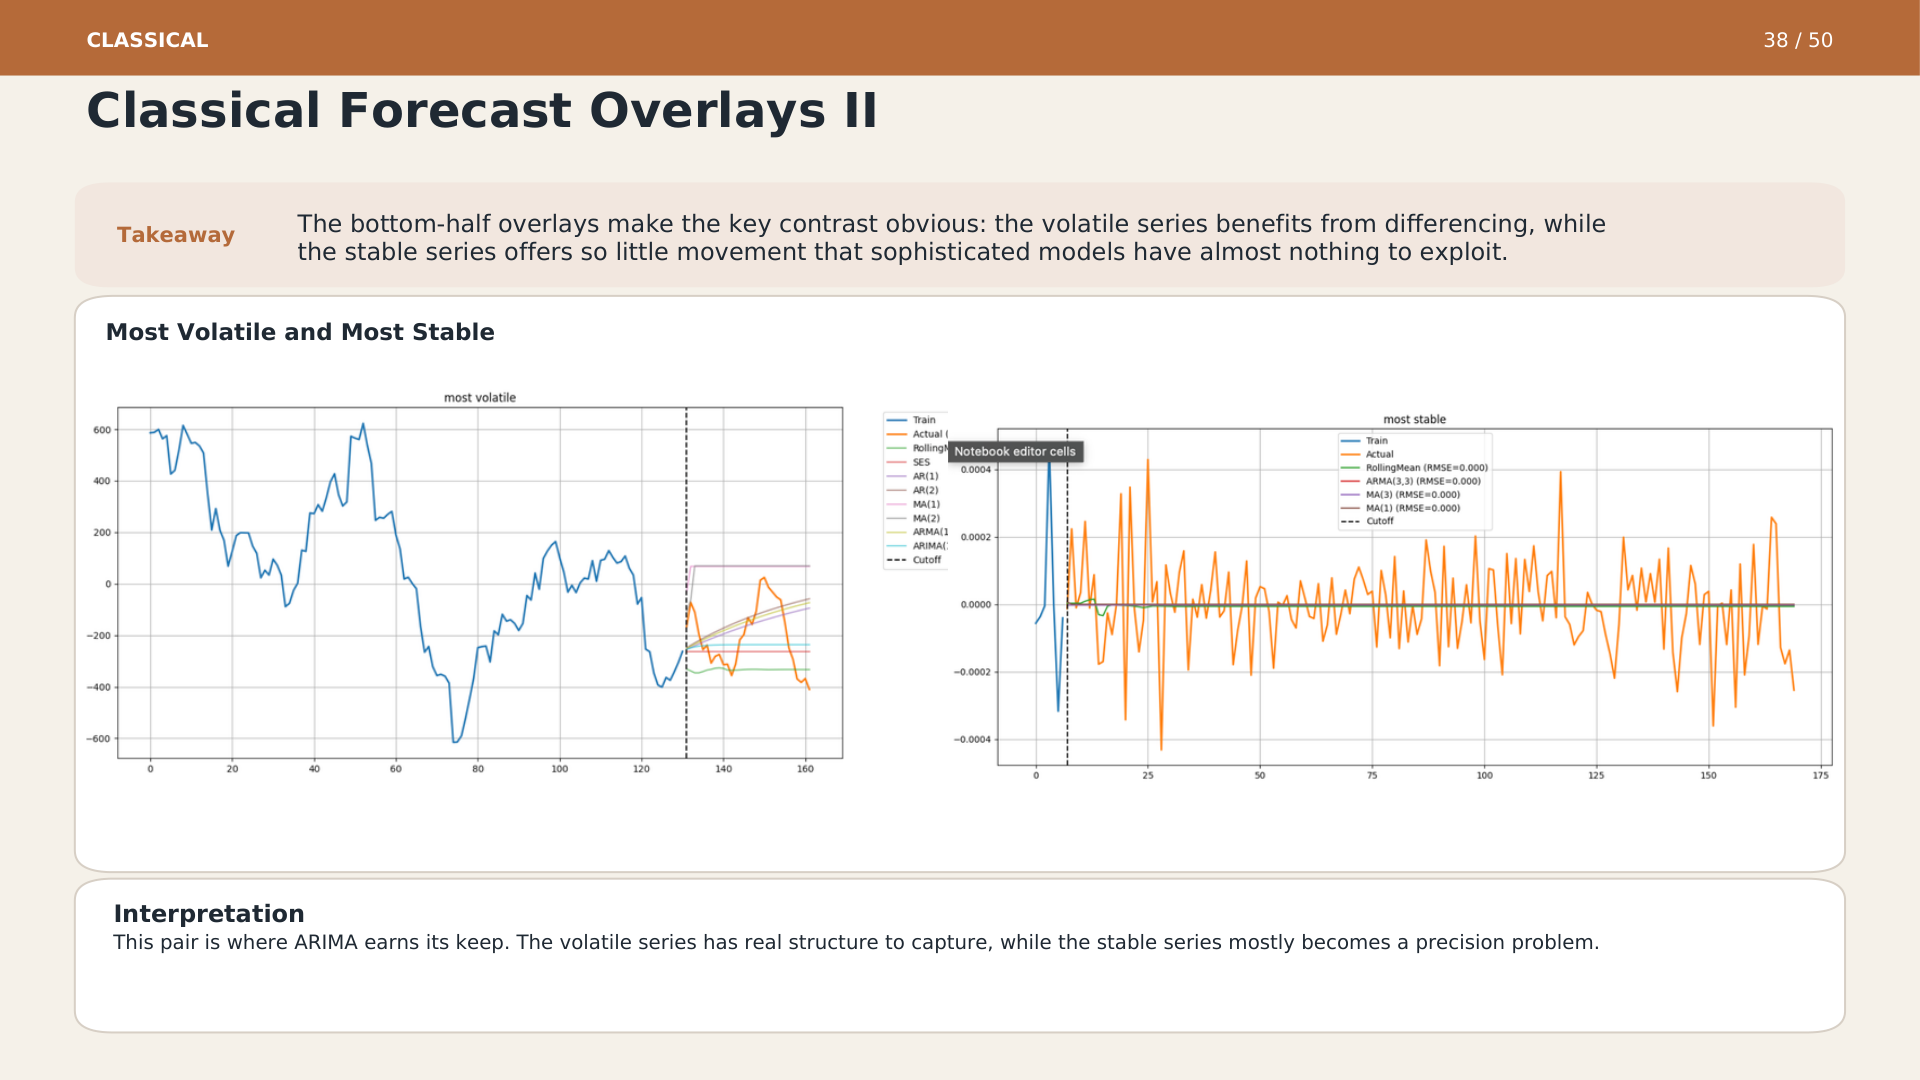
\includegraphics[width=0.95\textwidth]{figures/slide_34.png}
\caption{Classical forecast overlays for the most volatile and most stable representative series. The volatile series benefits from differencing---AR(1) captures short-lag persistence---while the stable series offers so little movement that sophisticated models have almost nothing to exploit.}
\label{fig:classical_forecasts}
\end{figure}

\begin{figure}[H]
\centering
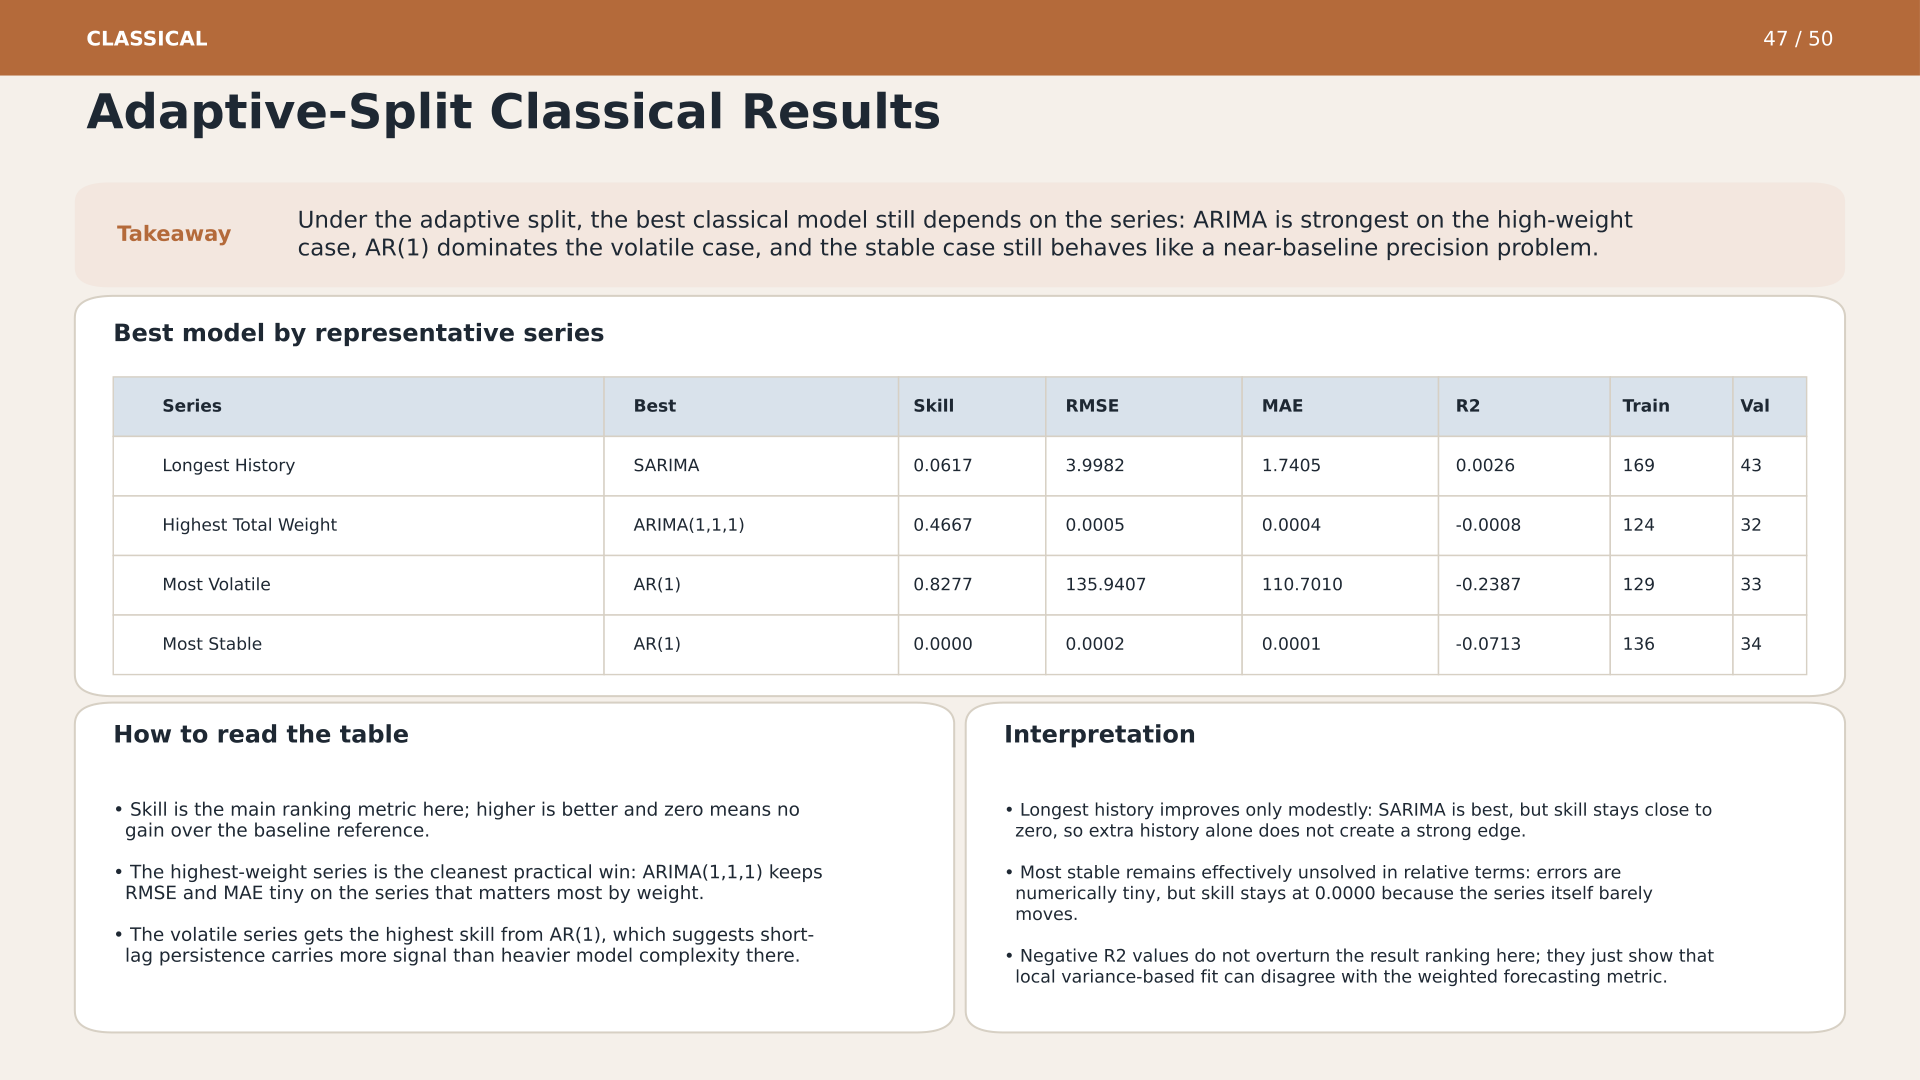
\includegraphics[width=0.95\textwidth]{figures/slide_38.png}
\caption{Adaptive-split classical results. Per-series best models: SARIMA wins on the longest-history series (skill 0.06), ARIMA(1,1,1) is strongest on the high-weight case (skill 0.47), AR(1) dominates both the volatile (skill 0.83) and stable (skill 0.00) cases. The volatile series has the most exploitable structure.}
\label{fig:classical_results}
\end{figure}

\subsubsection{The Stationarity Validation}

The $d=0$ versus $d=1$ comparison provides empirical validation of the EDA's stationarity finding:

\begin{itemize}
    \item Across matched-order pairs (e.g., ARIMA(1,0,0) vs. AR(1) $\equiv$ ARIMA(1,1,0)), the $d=1$ variant wins on the majority of series.
    \item This confirms that first differencing is genuinely beneficial for this dataset, not just a theoretical assumption.
\end{itemize}

\subsection{Deep Learning Performance Summary}

The three recurrent architectures generally show:

\begin{itemize}
    \item \textbf{LSTM and GRU} tend to outperform vanilla RNN, consistent with their superior gradient flow properties.
    \item Performance varies considerably across series, with some series showing substantial improvement over classical baselines and others showing degradation.
    \item Error accumulation in recursive forecasting is a significant factor, particularly for longer validation horizons.
\end{itemize}

\begin{figure}[H]
\centering
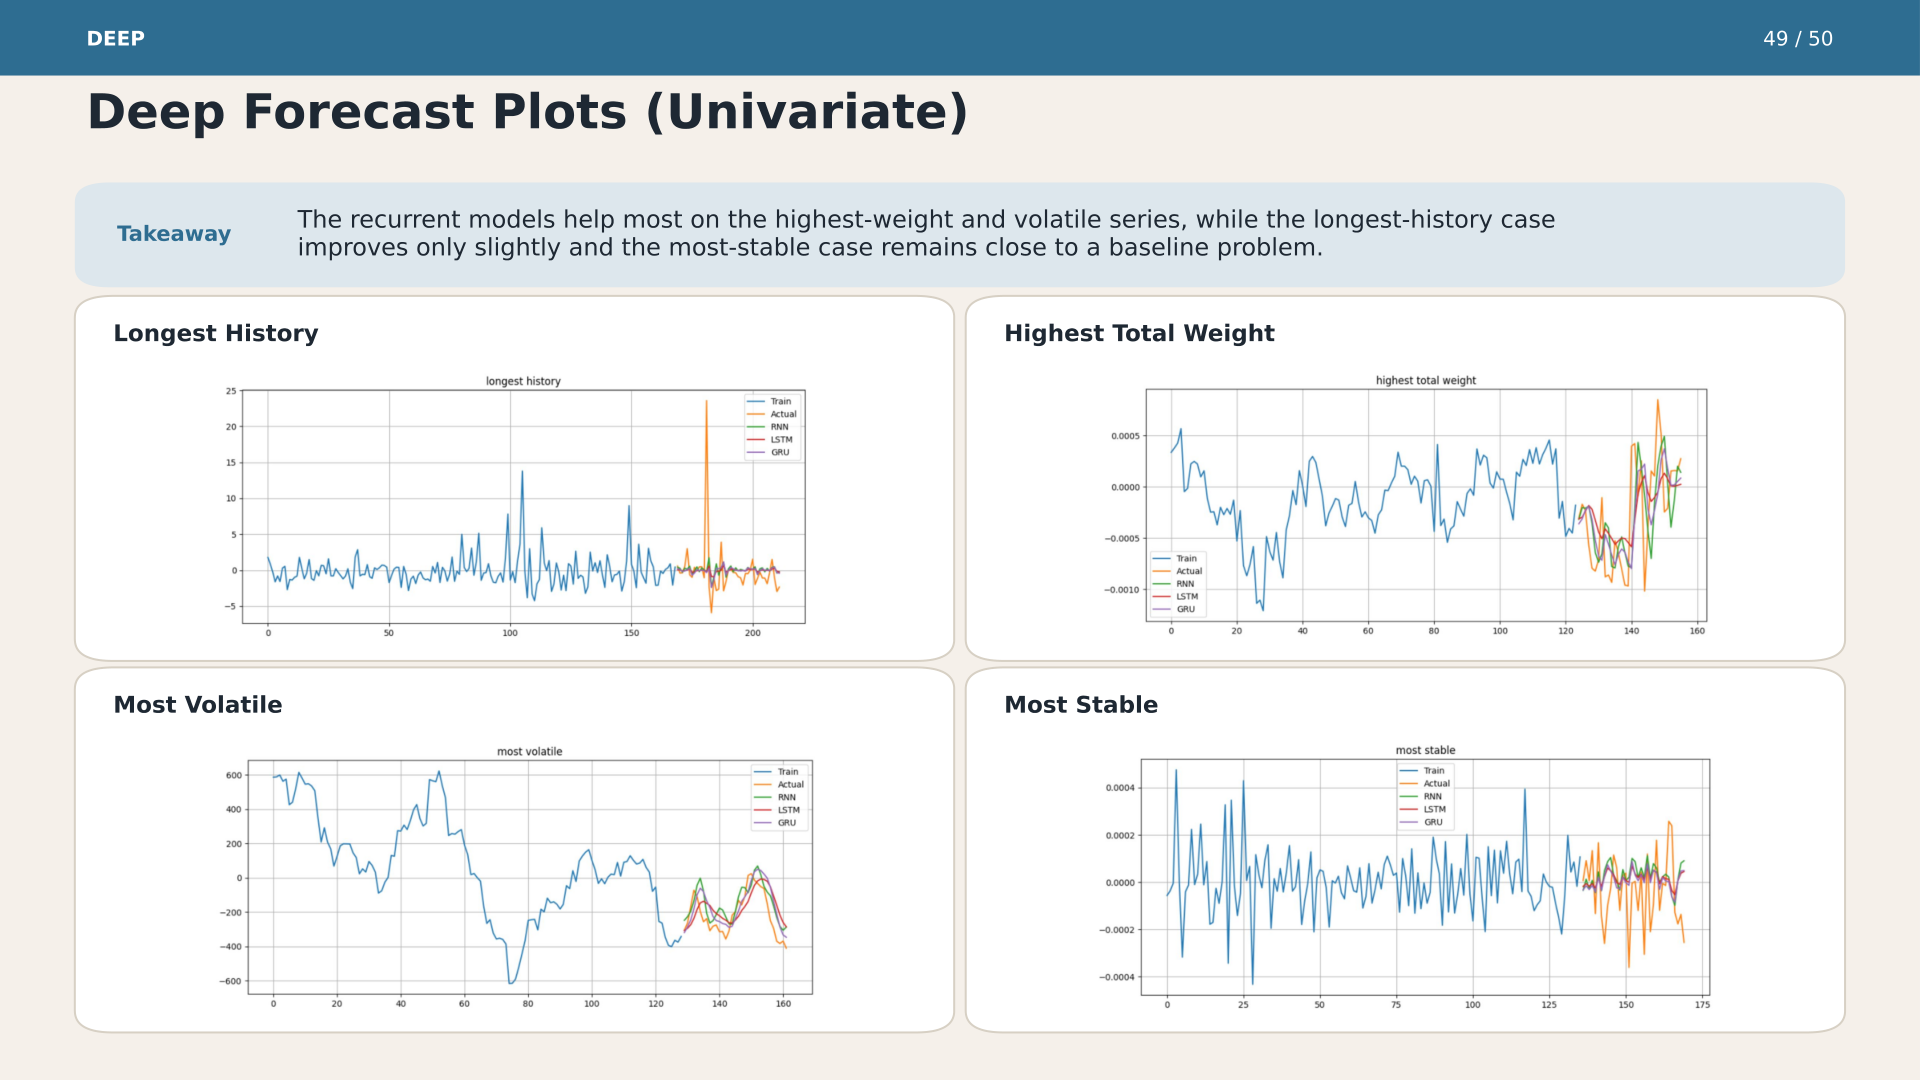
\includegraphics[width=0.95\textwidth]{figures/slide_40.png}
\caption{Deep forecast plots (univariate) for four representative series. The recurrent models help most on the highest-weight and volatile series, while the longest-history case improves only slightly and the most-stable case remains close to a baseline problem. Each panel shows Train (blue), Actual validation (orange), and overlaid RNN/LSTM/GRU predictions.}
\label{fig:deep_forecasts}
\end{figure}

\begin{figure}[H]
\centering
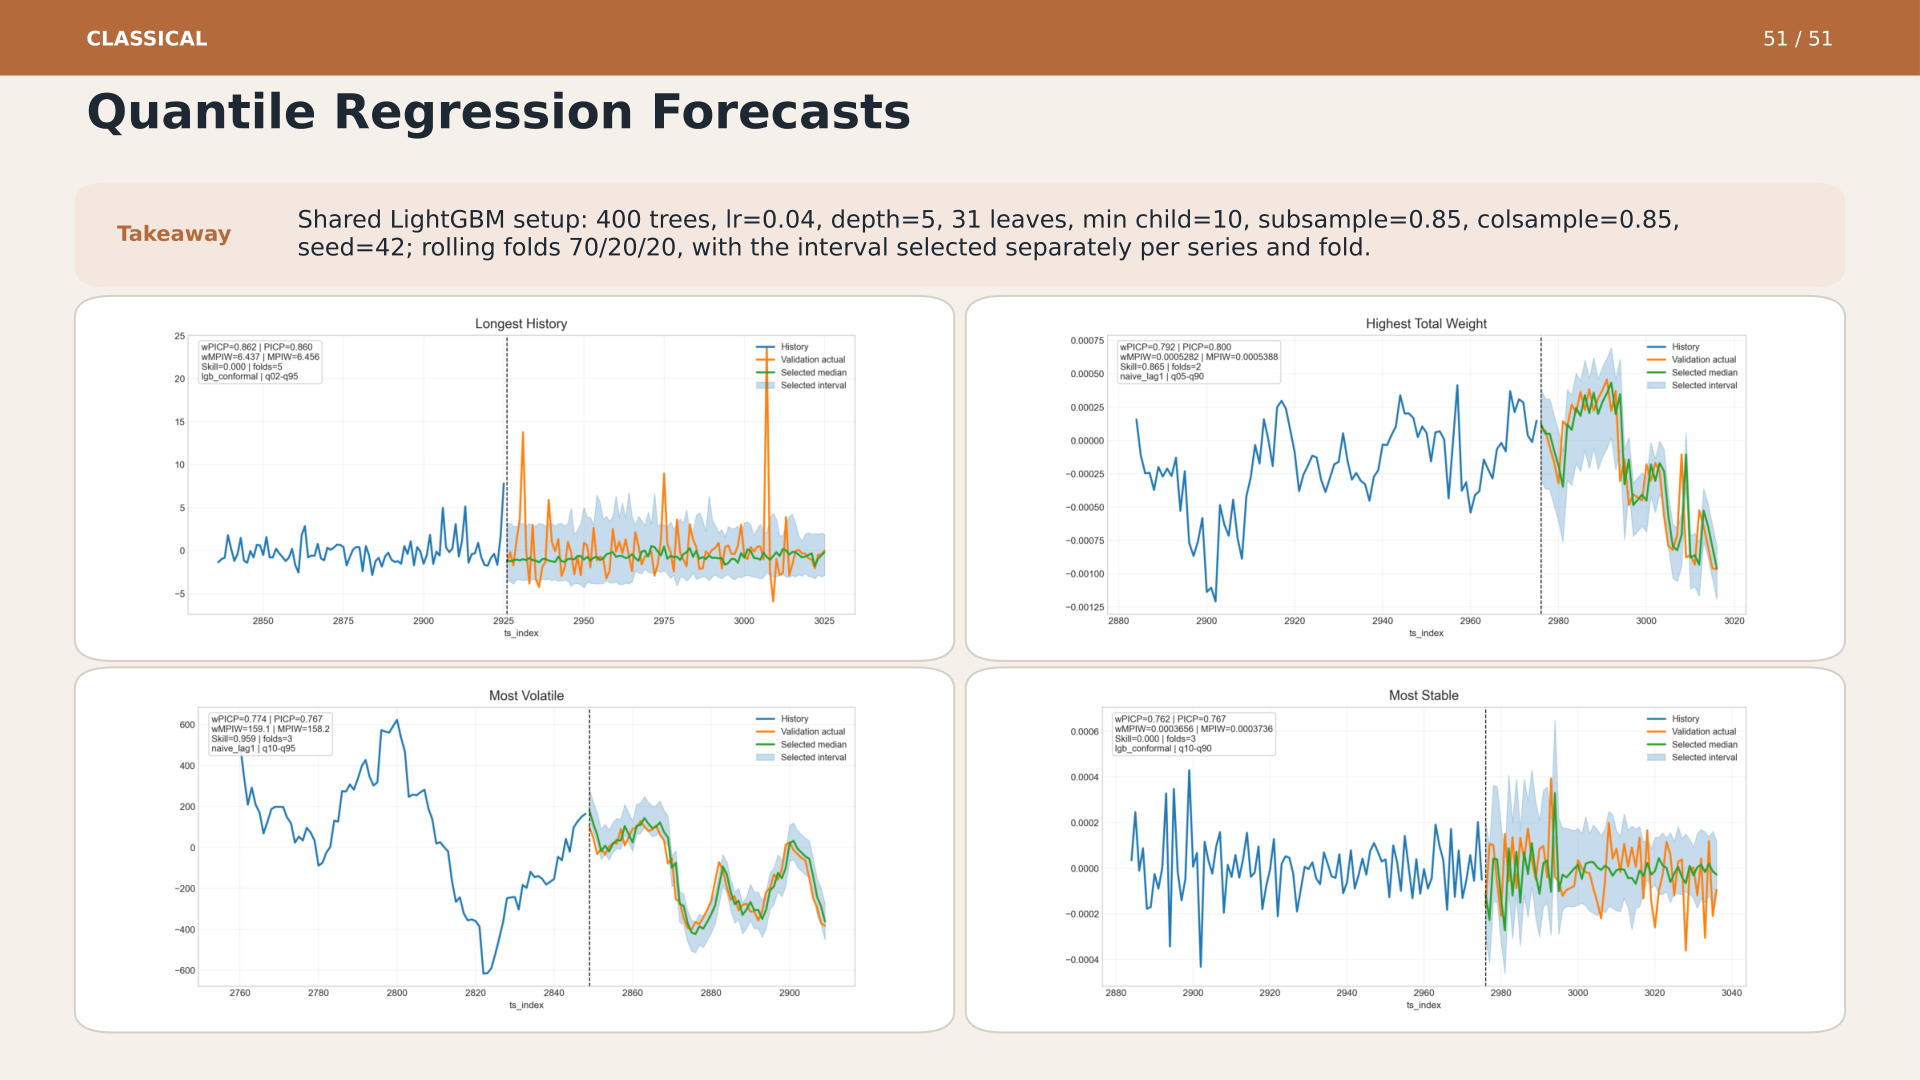
\includegraphics[width=0.95\textwidth]{figures/slide_42.png}
\caption{Quantile regression forecasts using LightGBM. Each panel shows the training history (blue), validation actuals (orange), selected median forecast (green), and prediction intervals (shaded blue). The model achieves PICP values between 0.76--0.86 across the four representative series.}
\label{fig:quantile_regression}
\end{figure}

\subsection{Classical vs. Deep Learning}

The relative performance of classical versus deep learning models depends on the characteristics of each series:

\begin{table}[H]
\centering
\caption{Conditions favoring each model family.}
\begin{tabularx}{\textwidth}{>{\raggedright\arraybackslash}X>{\raggedright\arraybackslash}X}
\toprule
\textbf{Classical Models Excel When} & \textbf{Deep Models Excel When} \\
\midrule
Series has strong, simple linear autocorrelation & Nonlinear temporal dependencies exist \\
Training data is limited & Sufficient training data is available \\
Short forecast horizons & Complex patterns justify the model complexity \\
Target is approximately Gaussian & Heavy tails require flexible modeling \\
\bottomrule
\end{tabularx}
\end{table}

\subsection{Key Findings}

\begin{enumerate}
    \item \textbf{No single model dominates.} The heterogeneous panel means different series favor different approaches, strongly motivating ensemble methods.

    \item \textbf{Simple baselines are hard to beat.} On many series, the Expanding Mean or Rolling Mean performs comparably to or better than complex models. This is characteristic of noisy financial data.

    \item \textbf{First differencing is essential.} The EDA's stationarity finding is empirically validated by the $d=0$ vs. $d=1$ comparison.

    \item \textbf{Weight concentration dominates scoring.} Because 65\% of the weighted score comes from 1\% of observations, models must perform well on these critical rows.

    \item \textbf{Feature-based models are needed.} The uniformly weak individual feature correlations ($|\rho| < 0.10$) suggest that signal resides in feature \emph{interactions}, which gradient-boosted trees or deeper neural networks could exploit.
\end{enumerate}

\subsection{Error Analysis}
\subsubsection{Common Failure Modes}

\begin{itemize}
    \item \textbf{Divergent forecasts:} ARIMA models fitted on levels ($d=0$) occasionally produce forecasts that diverge from the data range.
    \item \textbf{Outlier sensitivity:} The Drift model is particularly sensitive to outliers at the beginning or end of the training window.
    \item \textbf{Error accumulation:} Recursive forecasting in deep models degrades accuracy over longer horizons.
\end{itemize}

\subsubsection{Skip and Failure Analysis}

The 17.9\% skip rate in the classical pipeline is driven by:
\begin{itemize}
    \item SARIMA models (requiring 50--80 observations minimum)
    \item High-order AR/MA/ARMA models on short series
\end{itemize}

The near-zero failure rate (1 out of 8,200) indicates robust numerical implementation.

\subsection{Research Gap Identified}
\begin{enumerate}
    \item \textbf{Univariate only:} Classical models cannot exploit the 86 predictor features.
    \item \textbf{Linear assumptions:} AR/MA/ARMA/ARIMA assume linear relationships, missing nonlinear dynamics.
    \item \textbf{No cross-series learning:} Each series is modeled independently, ignoring potential shared structure across the panel.
    \item \textbf{Computational cost at scale:} Fitting 41 models on 1,930 series requires significant computation.
\end{enumerate}

These limitations motivate the deep learning approach in the next chapter.
\begin{enumerate}
    \item \textbf{Error accumulation:} Recursive forecasting compounds errors over long horizons. Direct multi-step forecasting could mitigate this.
    \item \textbf{Overfitting risk:} With many parameters and limited per-series data, overfitting is a concern. Regularization, dropout, and early stopping are essential.
    \item \textbf{Weight-aware training:} The current MSE loss does not incorporate observation weights. Implementing weighted loss would better align training with the competition metric.
    \item \textbf{Feature utilization:} The current implementation focuses on univariate forecasting. Incorporating the 86 predictor features could substantially improve performance.
    \item \textbf{Computational cost:} Training separate models per series is expensive. Global or meta-learning approaches could amortize this cost.
\end{enumerate}

